\documentclass[unicode,11pt,a4paper,oneside,numbers=endperiod,openany]{scrartcl}

\renewcommand{\thesubsection}{\arabic{subsection}}

\usepackage{listings}
\usepackage{xcolor}
\usepackage{float}
\usepackage{amsmath}
\usepackage{amsmath, amssymb} % for math symbols and fonts
\usepackage{hyperref} % for hyperlinks
\usepackage{graphicx} % for including images
\usepackage{subcaption} % for subfigures
\usepackage{booktabs} % for tables


\lstset{language=Matlab,%
    basicstyle=\color{red}\ttfamily\small,%
    breaklines=true,%
    morekeywords={matlab2tikz},%
    keywordstyle=\color{blue},%
    morekeywords=[2]{1}, keywordstyle=[2]{\color{black}},%
    identifierstyle=\color{black},%
    stringstyle=\color{mylilas},%
    commentstyle=\color{mygreen},%
    showstringspaces=false,%
    numbers=left,%
    numberstyle={\tiny \color{black}},% size of the numbers
    numbersep=9pt, % this defines how far the numbers are from the text
    emph=[1]{for,end,break},emphstyle=[1]\color{red}, %some words to emphasise
    emph=[2]{word1,word2}, emphstyle=[2]{style},%
}


\usepackage{ifthen}
\usepackage[utf8]{inputenc}
\usepackage{graphics}
\usepackage{graphicx}
\usepackage{hyperref}

\pagestyle{plain}
\voffset -5mm
\oddsidemargin  0mm
\evensidemargin -11mm
\marginparwidth 2cm
\marginparsep 0pt
\topmargin 0mm
\headheight 0pt
\headsep 0pt
\topskip 0pt        
\textheight 255mm
\textwidth 165mm

\newcommand{\duedate} {}
\newcommand{\setduedate}[1]{%
\renewcommand\duedate {\textbf{Due date:}~ #1}}
\newcommand\isassignment {false}
\newcommand{\setassignment}{\renewcommand\isassignment {true}}
\newcommand{\ifassignment}[1]{\ifthenelse{\boolean{\isassignment}}{#1}{}}
\newcommand{\ifnotassignment}[1]{\ifthenelse{\boolean{\isassignment}}{}{#1}}

\newcommand{\assignmentpolicy}{
\begin{table}[h]
\begin{center}
\scalebox{0.8} {%
\begin{tabular}{|p{0.02cm}p{16cm}|}
\hline
&\\
\multicolumn{2}{|c|}{\Large\textbf{Numerical Computing 2023 ---  Submission Instructions}}\\
\multicolumn{2}{|c|}{\large\textbf{(Please, notice that following instructions are mandatory: }}\\
\multicolumn{2}{|c|}{\large\textbf{submissions that don't comply with, won't be considered)}}\\
&\\
\textbullet & Assignments must be submitted to \href{https://www.icorsi.ch/course/view.php?id=14666}{iCorsi} (i.e. in electronic format).\\
\textbullet & Provide both executable package and sources (e.g. C/C++ files, MATLAB). 
If you are using libraries, please add them in the file. Sources must be organized in directories called:\\
\multicolumn{2}{|c|}{\textit{Project\_number\_lastname\_firstname}}\\
& and  the  file must be called:\\
\multicolumn{2}{|c|}{\textit{project\_number\_lastname\_firstname.zip}}\\
\multicolumn{2}{|c|}{\textit{project\_number\_lastname\_firstname.pdf}}\\
\textbullet &  The TAs will grade your project by reviewing your project write-up, and looking at the implementation you attempted, and benchmarking your code's performance.\\

\textbullet & You are allowed to discuss all questions with anyone you like; however: (i) your submission must list anyone you discussed problems with and (ii) you must write up your submission independently.\\
\hline
\end{tabular}
}
\end{center}
\end{table}
}
\newcommand{\punkte}[1]{\hspace{1ex}\emph{\mdseries\hfill(#1~\ifcase#1{Points}\or{Points}\else{Points}\fi)}}


\newcommand\serieheader[6]{
\thispagestyle{empty}%
\begin{flushleft}

\includegraphics[width=0.45\textwidth]{CI_logo}
\end{flushleft}
  \noindent%
  {\large\ignorespaces{\textbf{#1}}\hspace{\fill}\ignorespaces{ \textbf{#2}}}\\ \\%
  {\large\ignorespaces #3 \hspace{\fill}\ignorespaces #4}\\
  \noindent%
  \bigskip
  \hrule\par\bigskip\noindent%
  \bigskip {\ignorespaces {\Large{\textbf{#5}}}
  \hspace{\fill}\ignorespaces \large \ifthenelse{\boolean{\isassignment}}{\duedate}{#6}}
  \hrule\par\bigskip\noindent%  \linebreak
 }

\makeatletter
\def\enumerateMod{\ifnum \@enumdepth >3 \@toodeep\else
      \advance\@enumdepth \@ne
      \edef\@enumctr{enum\romannumeral\the\@enumdepth}\list
      {\csname label\@enumctr\endcsname}{\usecounter
        {\@enumctr}%%%? the following differs from "enumerate"
	\topsep0pt%
	\partopsep0pt%
	\itemsep0pt%
	\def\makelabel##1{\hss\llap{##1}}}\fi}
\let\endenumerateMod =\endlist
\makeatother




\usepackage{textcomp}





\begin{document}


\setassignment
\setduedate{Wednesday, 8 November 2023, 11:59 PM}

\serieheader{Numerical Computing}{2023}{\textbf{Student:} Harkeerat Singh Sawhney}{}
\newline

\assignmentpolicy


\newpage

\subsection{Spectral clustering of non-convex sets [50 points]}

\subsubsection{}

\begin{figure}[H]
    \centering
    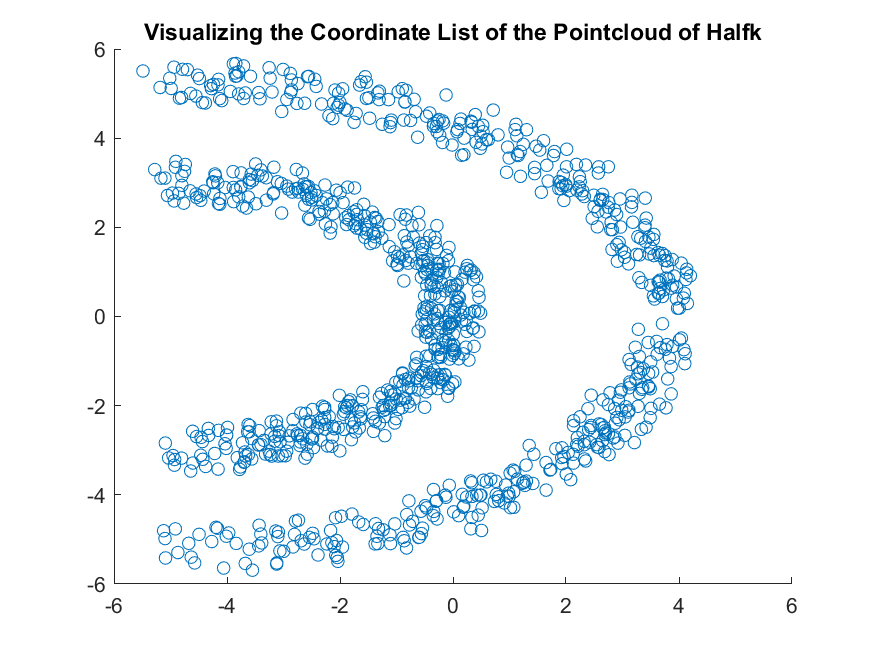
\includegraphics[width=0.5\textwidth]{figures/1.1.png}
    \caption{Plot of the data points for HalfK}
    \label{fig:1.1}
\end{figure}

Figure \ref{fig:1.1} shows the plot of the data points for HalfK. By observing the figure we can easily see the two clusters in the data. The two clusters are half a circle, in which one is within the other. It is easy for us to look at the graph and distinguish the two clusters, but it is not easy for different algorithms to do the same. There are 2 different approaches which this project focuses on; K-Means and Spectral Clustering.
\\ \\
The K-Means Algorithm takes identifies the two clusters by taking the mean of the two clusters and then assigning the points to the cluster which is the closes to the point. In the other Spectral Clustering is a modified version of K-Means clustering which runs the algorithm on the eigenvectors of the graph's Laplacian Matrix and adjusts the cluster centroids based on its Eigenvectors coordinates. As it can be noticed that calculating the Eigenvectors and Eigenvalues of the Laplacian Matrix is computationally expensive as compare to the K-Means algorithm.
\\ \\
If theoretically both the algorithms run over the data points of HalfK, we should observe different results. K-Means with Spectral method should be able to properly identify the two clusters, but K-Means without Spectral method should not be able to identify the two clusters. This is because the data points are not linearly separable and the original K-Means algorithm would not be able to do the same in this case. The reason is because it uses Euclidean Distance. With the use of Euclidean Distance the data points in each cluster are modeled by the position of their centroids, in which K-Means assumes all clusters should have the same radius. Hence because of this assumption, the K-Means algorithm would not be able to identify proper clusters in Spherical data. In the following questions this theory will be tested.

\subsubsection{Computing $\in$ Factor}
The points are all in the space and we need a function which lets us define them and compute the similarity of any 2 points. Hence the function which would be used to compute the similarity of any 2 points would be Gaussian Kernel Similarity Function. The function is as follows:
\begin{equation}
    s(x_i, x_j) = e^{-\frac{||x_i - x_j||^2}{2\sigma^2}}
\end{equation}

The Gaussian Kernel Similarity Function tends to be between 0 and 1. In the function the choice of the $\sigma$ is very important as it controls how big or small the neighborhood of a point is. In our case we chose the given value which is $log(n)$.

Once the Gaussian Kernel Similarity Function is defined, we can then compute the Minimal Spanning Tree so that we can remove any edges which are not required. With this we can at last chose our $\in$ factor. The $\in$ factor is the maximum spanning tree of the Gaussian Similarity. In table \ref{tab:in-factor} we can see the $\in$ factor for each of the data sets.

\begin{table}[H]
    \centering
    \begin{tabular}{|l|c|}
        \hline
        \textbf{Mesh}         & \textbf{$\in$ Factor} \\
        \hline
        Two Spirals           & 0.6883                \\
        Cluster in Cluster    & 0.63243               \\
        Crescent \& Full Moon & 0.55984               \\
        Corn                  & 0.55469               \\
        Outliers              & 0.29756               \\
        \hline
    \end{tabular}
    \caption{The $\in$ factor for each of the data sets}
    \label{tab:in-factor}
\end{table}

\subsubsection{$\in$ Similarity Graph}
We are asked to complete the Matlab Function \textit{epsilonSimGraph()} which takes in the data points and the $\in$ factor and returns the $\in$ Similarity Graph. We can utilize the Pseudo Code given in the lecture notes to complete the function. The function is as follows:

\begin{lstlisting}
n = size(Pts,1);
G = zeros(n,n);

for i = 1:n
    for j = 1:n
        distance = norm(Pts(i,:) - Pts(j,:));
        if distance < epsilon
            G(i, j) = 1;
        end
    end
end    
\end{lstlisting}

In the above code we are iterating over all the points and calculating the distance between them. If the distance is less than the $\in$ factor then we are adding an edge between the two points. The function returns the $\in$ Similarity Graph.

\subsubsection{Adjacency Matrix for the $\in$ Similarity Graph}
In order to get the Adjacency Matrix we just need to multiply the $\in$-neighborhood Graph with the Gaussian Similarity Matrix.

\begin{equation}
    S \odot G = W
\end{equation}

From this we can graph the resulting Adjacency Matrix. The Adjacency Matrix for the $\in$ Similarity Graph for each of the data sets is shown in figure \ref{fig:1.4}.

\begin{figure}[H]
    \centering
    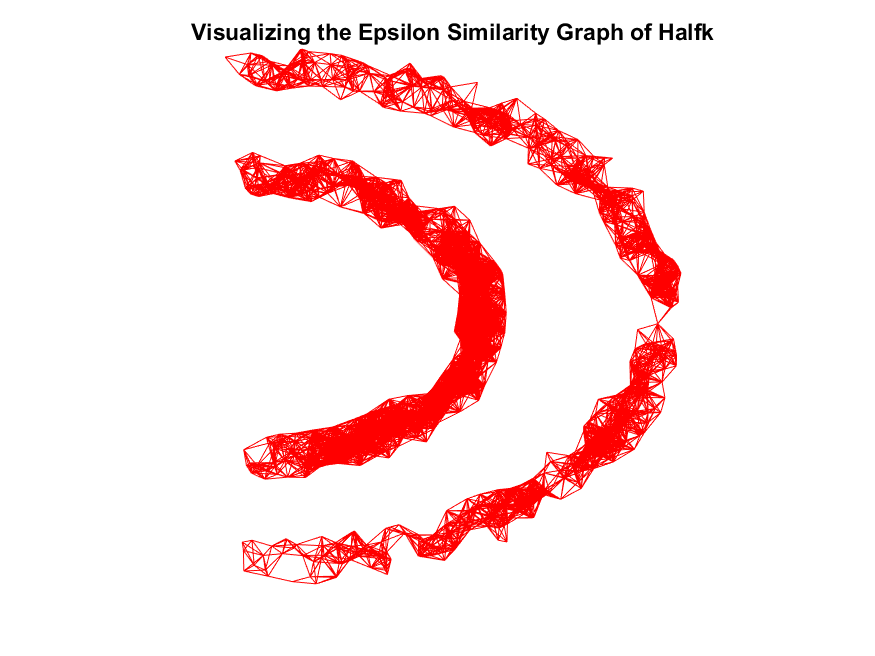
\includegraphics[width=0.5\textwidth]{figures/1.4.png}
    \caption{Adjacency Matrix for the $\in$ Similarity Graph}
    \label{fig:1.4}
\end{figure}

\subsubsection{Laplacian Matrix for the $\in$ Similarity Graph and Spectral Clustering}

In order to obtain the Laplacian Matrix, we utilize the function \textit{CreateLapl}, which takes the Adjacency Matrix as input and returns the Laplacian Matrix. Next, we compute the Eigenvalues and Eigenvectors of the Laplacian Matrix, sort the Eigenvalues in ascending order, and select the K smallest Eigenvalues (which can be either 2 or 4) along with their corresponding Eigenvectors. We then pass these selected Eigenvectors to the \textit{kmeansMod} function, which returns the clusters. Finally, we visualize these clusters by plotting them on the graph.

Bellow is also the code for the Spectral Clustering algorithm.

\begin{lstlisting}
[L, Diag] = CreateLapl(W);
[V, D] = eig(L);

lambda = diag(D);
[lambda, idx] = sort(lambda);
Y = V(:,idx(1:K));

[D_spec,x_spec] = kmeans_mod(Y, K, n);
\end{lstlisting}

\subsubsection{Visualization of Two Clustering Algorithms}

\begin{figure}[H]
    \centering
    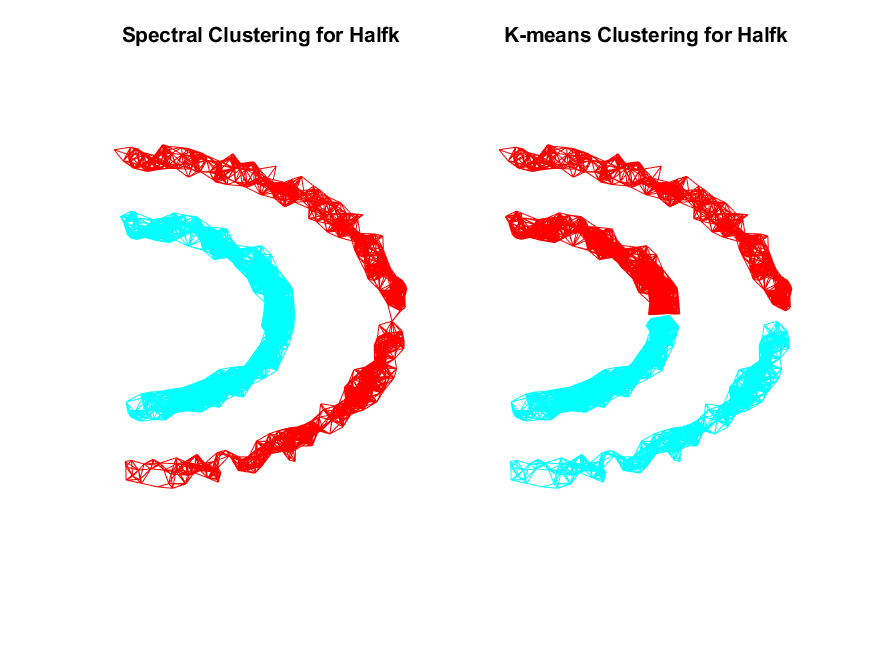
\includegraphics[width=0.5\textwidth]{figures/1.7.png}
    \caption{Spectral Clustering and K-Means Clustering on HalfK}
    \label{fig:1.7}
\end{figure}

In Figure \ref{fig:1.7}, we can see that the Spectral Clustering algorithm is able to identify the two clusters in the data set while the K-Means algorithm is not able to accomplish that. This is mainly due to the reasons mentioned in the Question 1.1.

\subsubsection{Spectral Clustering and K-Means Clustering on Different Data Sets}
This is very similar to the previous question, but instead of using the HalfK data set we are using the other data sets.

\begin{figure}[H]
    \centering
    \begin{subfigure}{0.5\textwidth}
        \centering
        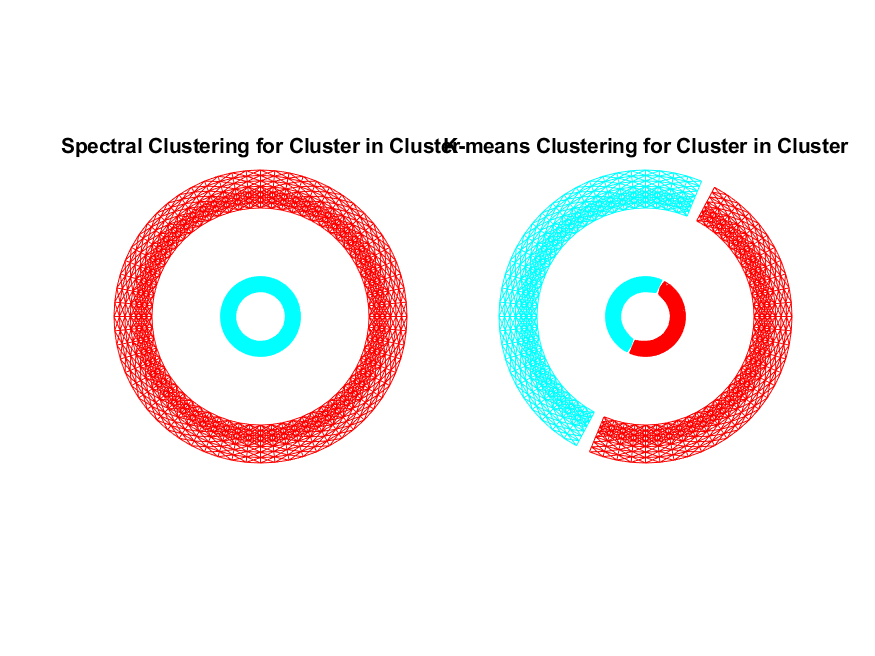
\includegraphics[width=\linewidth]{figures/1.7_Cluster in Cluster.png}
        \caption{Cluster in Cluster}
        \label{fig:cluster-in-cluster}
    \end{subfigure}
    \begin{subfigure}{0.5\textwidth}
        \centering
        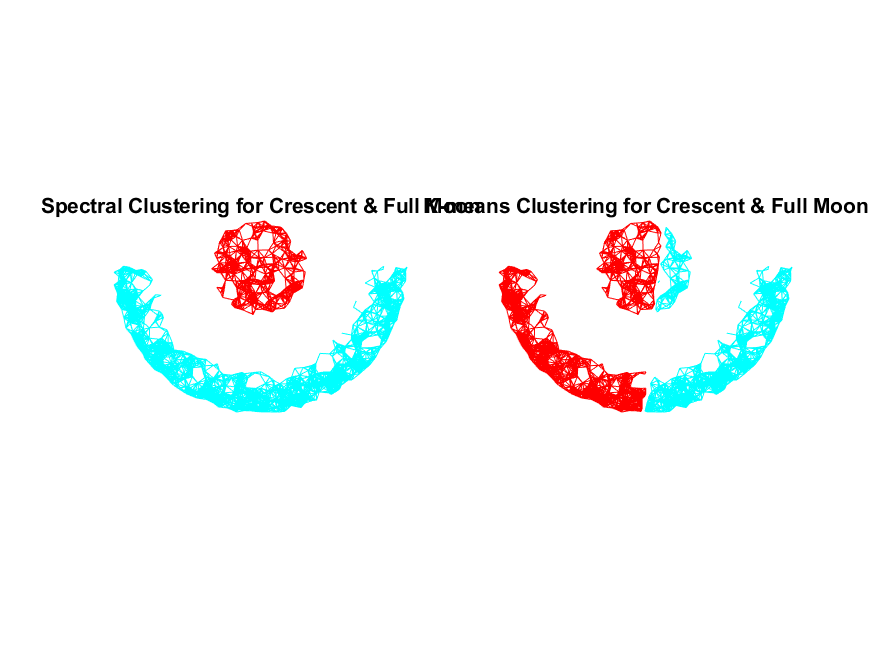
\includegraphics[width=\linewidth]{figures/1.7_Crescent & Full Moon.png}
        \caption{Crescent \& Full Moon}
        \label{fig:crescent-full-moon}
    \end{subfigure}
    \begin{subfigure}{0.5\textwidth}
        \centering
        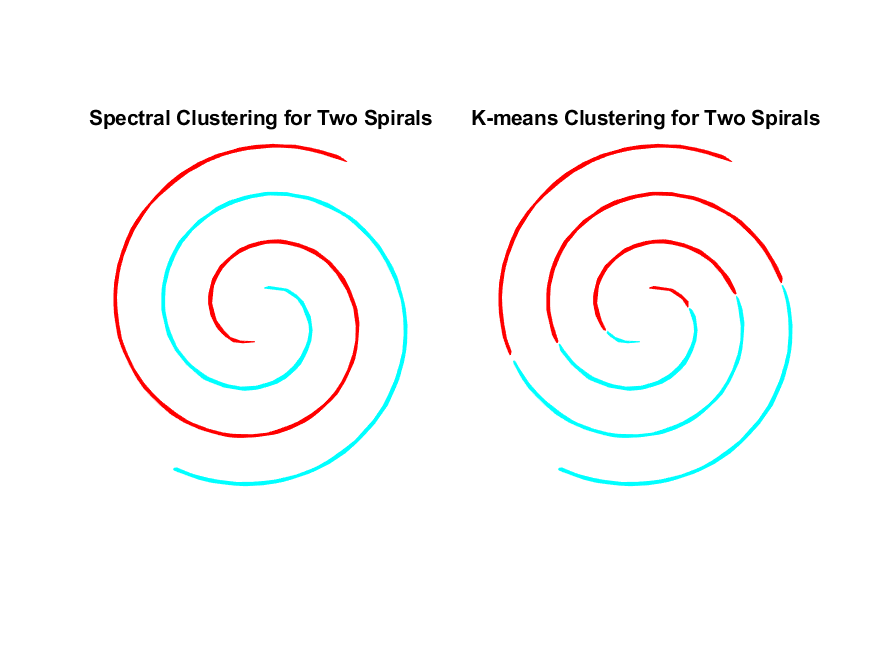
\includegraphics[width=\linewidth]{figures/1.7_Two Spirals.png}
        \caption{Two Spirals}
        \label{fig:two-spirals}
    \end{subfigure}
    \caption{Spectral Clustering and K-Means Clustering on Different Datasets}
    \label{fig:overall1}
\end{figure}


\begin{figure}[H]
    \centering
    \begin{subfigure}{0.5\textwidth}
        \centering
        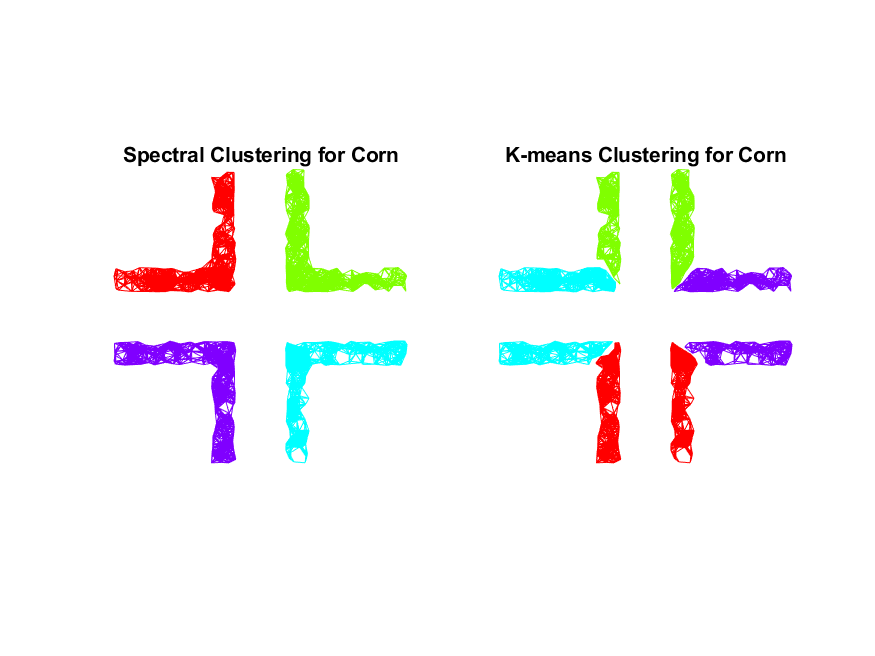
\includegraphics[width=\linewidth]{figures/1.7_Corn.png}
        \caption{Corn}
        \label{fig:corn}
    \end{subfigure}
    \begin{subfigure}{0.5\textwidth}
        \centering
        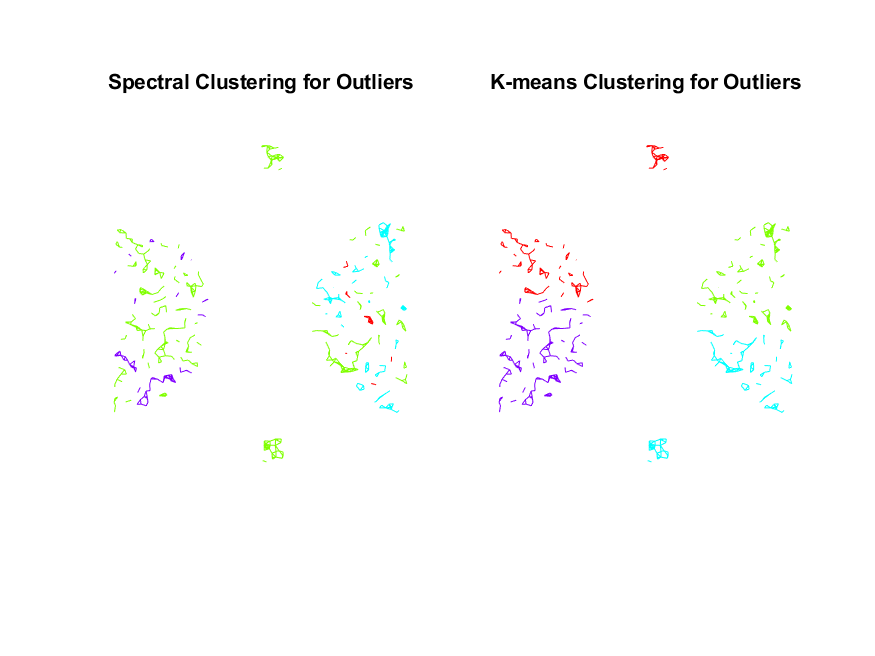
\includegraphics[width=\linewidth]{figures/1.7_Outliers.png}
        \caption{Outliers}
        \label{fig:outliers}
    \end{subfigure}
    \caption{Spectral Clustering and K-Means Clustering on K = 4}
    \label{fig:overall2}
\end{figure}

From the Figure \ref{fig:overall1} and Figure \ref{fig:overall2} we can see that the Spectral Clustering algorithm is able to identify the clusters in the data set while the K-Means algorithm is not able to accomplish the same that well. We can see for K = 4 that when there outliers it influences the centroid very heavily for K-Means Clustering. We also notice that K-Means Clustering treats all the centroids as the same size as it does not recognize the density of the clusters.


\subsection{Spectral clustering of real-world graphs [35 points]}

\subsubsection{Construction of Laplacian Matrix and Visualization of the Graph}
In this question we do everything the same as the Question 1.5, except that once we get the eigenvectors we take the 2nd and 3rd smallest eigenvectors. We then combine them into the matrix which is passed on to the \textit{kmeansMod} function. The code for this is as follows:

\begin{lstlisting}
lambda = diag(D);
[lambda, idx] = sort(lambda);
Y = V(:, idx(1:K));

v2 = Y(:,2);
v3 = Y(:,3);

new_coords = [v2, v3];
\end{lstlisting}

\begin{figure}[H]
    \centering
    \begin{subfigure}{0.45\textwidth}
        \centering
        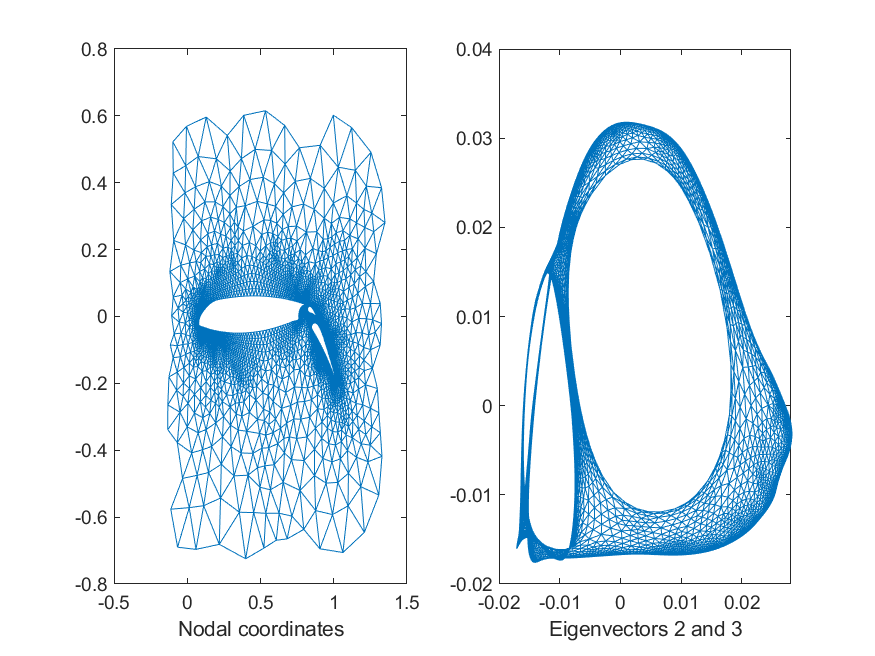
\includegraphics[width=\linewidth]{figures/2.1_airfoil1.png}
        \caption{Airfoil1}
        \label{fig:airfoil1}
    \end{subfigure}
    \hfill
    \begin{subfigure}{0.45\textwidth}
        \centering
        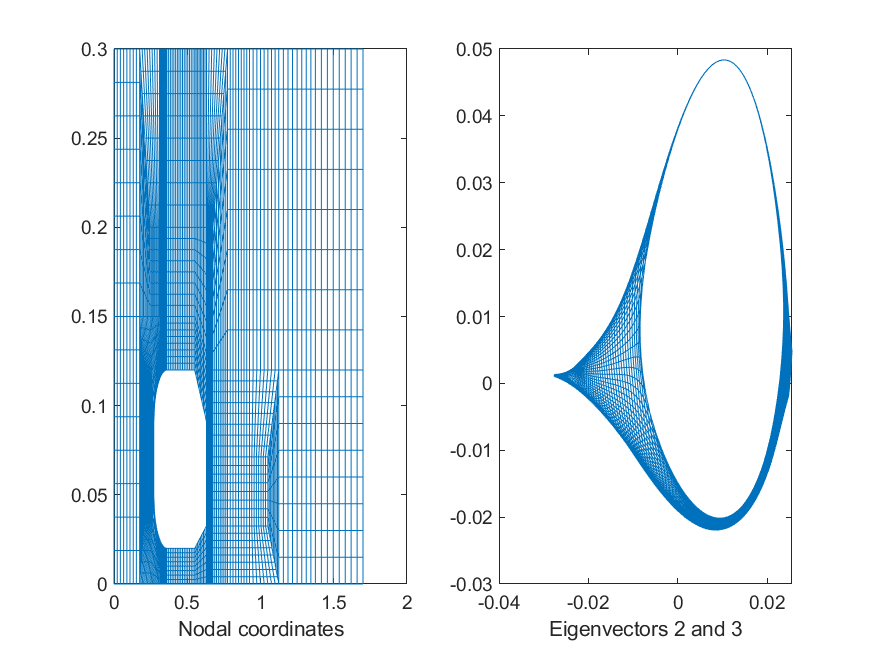
\includegraphics[width=\linewidth]{figures/2.1_grid2.png}
        \caption{Grid2}
        \label{fig:grid2}
    \end{subfigure}

    \begin{subfigure}{0.45\textwidth}
        \centering
        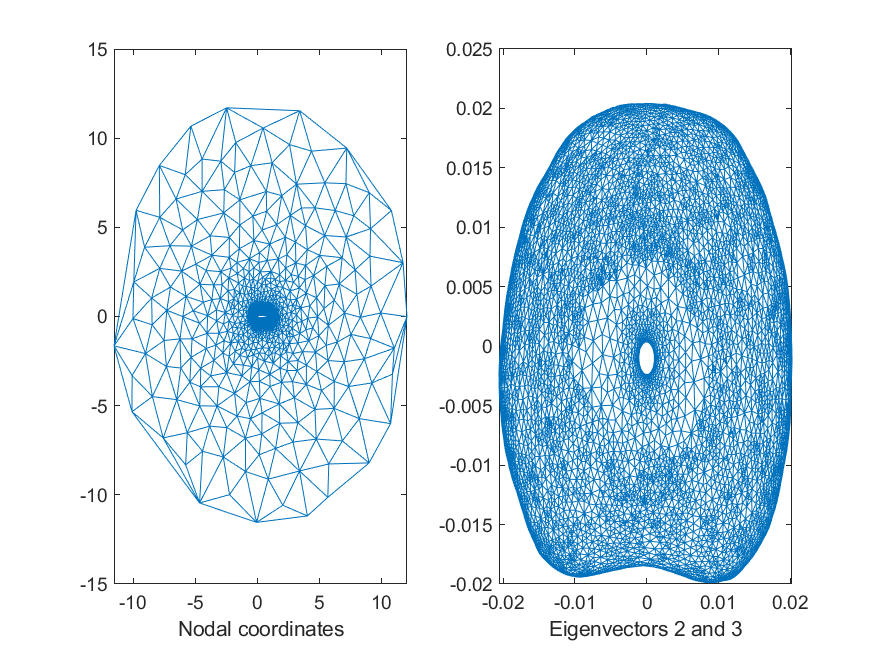
\includegraphics[width=\linewidth]{figures/2.1_barth.png}
        \caption{Barth}
        \label{fig:barth}
    \end{subfigure}
    \hfill
    \begin{subfigure}{0.45\textwidth}
        \centering
        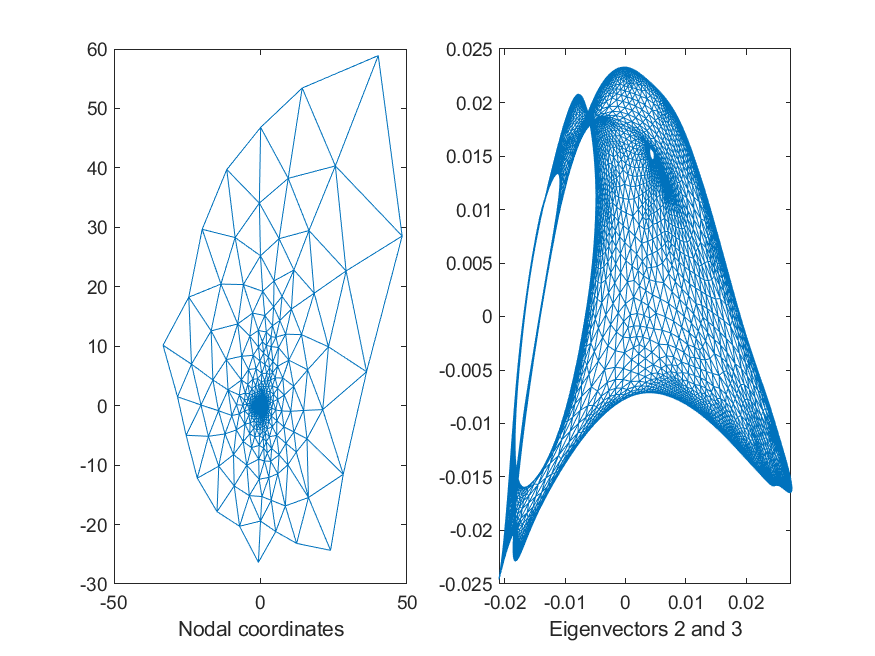
\includegraphics[width=\linewidth]{figures/2.1_3elt.png}
        \caption{3elt}
        \label{fig:3elt}
    \end{subfigure}
    \caption{Visualization of Different Graphs for Airfoil}
    \label{fig:overall3}
\end{figure}

In the Figure \ref{fig:overall3} we can see the visualization of the graph. We can see that it is visualized in two ways, one being with Nodal Coordinates and other being with the 2nd and 3rd smallest eigenvectors.

\subsubsection{Spectral Clustering and K-Means Clustering on Different Meshes}
In this question we are asked to run the Spectral Clustering and K-Means Clustering on the different meshes.

\begin{figure}[H]
    \centering
    \begin{subfigure}{0.45\textwidth}
        \centering
        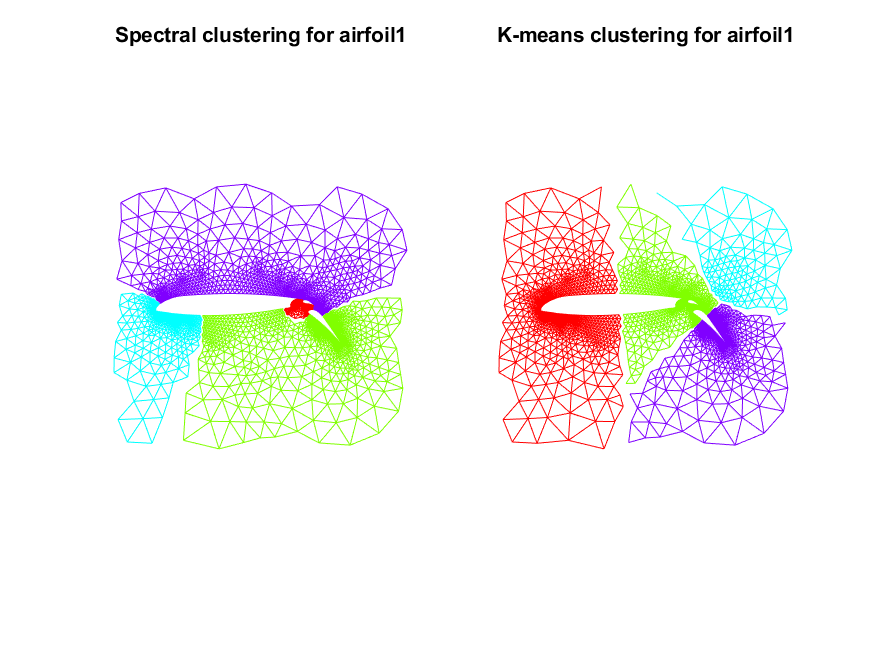
\includegraphics[width=\linewidth]{figures/2.2_airfoil1.png}
        \caption{Airfoil1}
        \label{fig:airfoil1-2.2}
    \end{subfigure}
    \hfill
    \begin{subfigure}{0.45\textwidth}
        \centering
        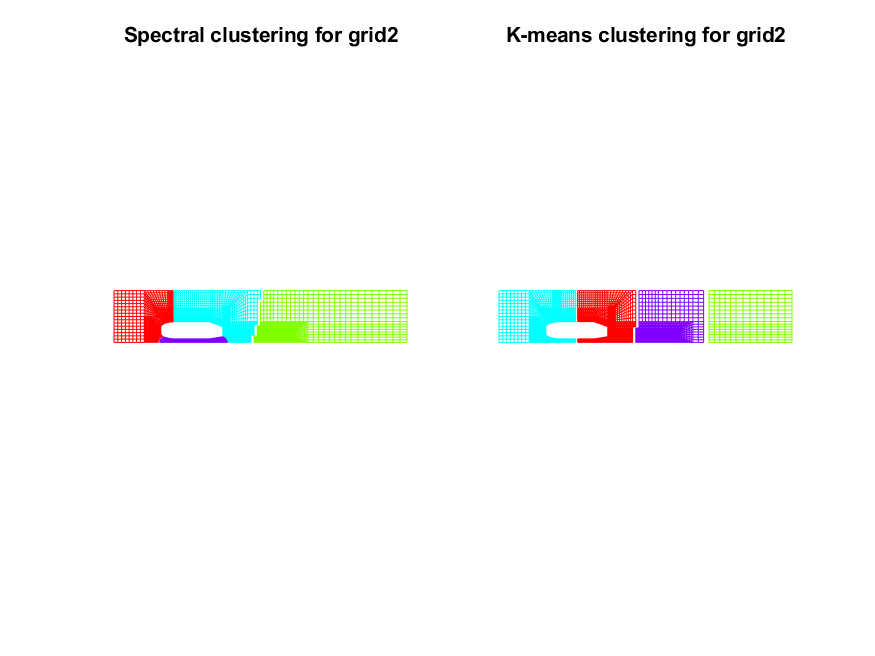
\includegraphics[width=\linewidth]{figures/2.2_grid2.png}
        \caption{Grid2}
        \label{fig:grid2-2.2}
    \end{subfigure}

    \begin{subfigure}{0.45\textwidth}
        \centering
        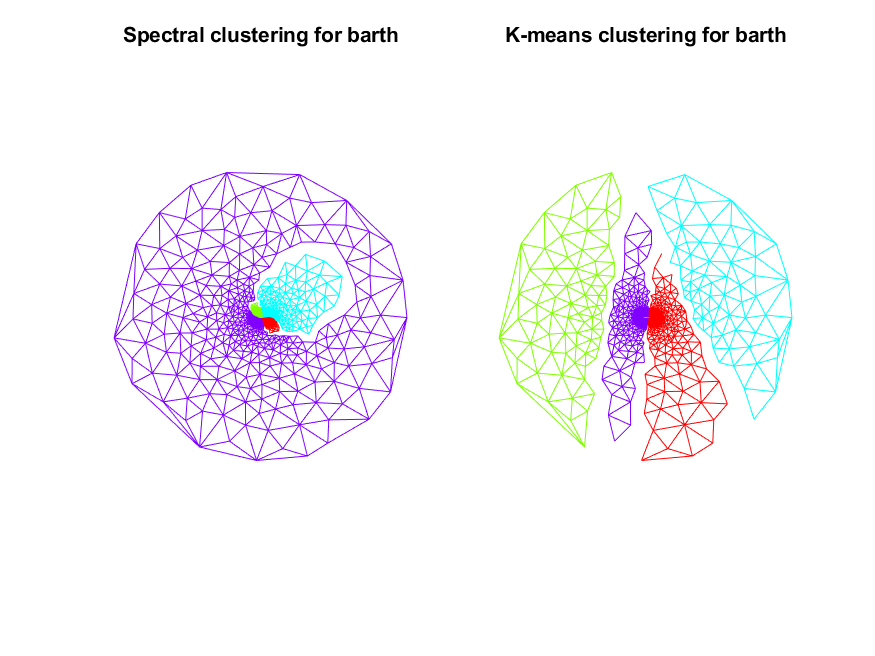
\includegraphics[width=\linewidth]{figures/2.2_barth.png}
        \caption{Barth}
        \label{fig:barth-2.2}
    \end{subfigure}
    \hfill
    \begin{subfigure}{0.45\textwidth}
        \centering
        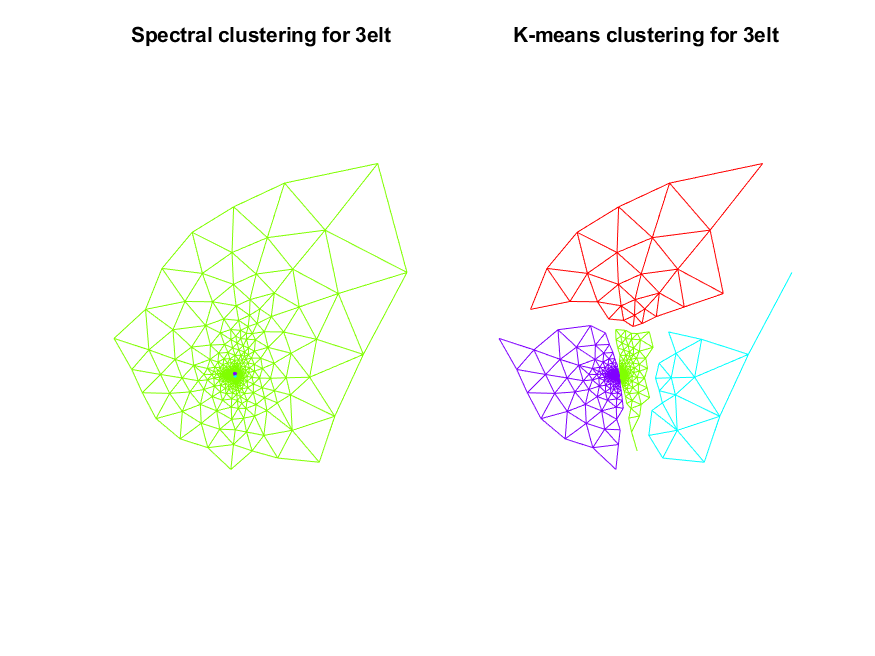
\includegraphics[width=\linewidth]{figures/2.2_3elt.png}
        \caption{3elt}
        \label{fig:3elt-2.2}
    \end{subfigure}
    \caption{Spectral Clustering and K-Means Clustering on Different Meshes}
    \label{fig:overall-2.2}
\end{figure}

\subsubsection{Visualization of Tables and Histograms}
What we can observe from all the data collected is that K-Means clustering fails to identify the Cluster Density and uses it partitioning based on the distance between points on their spatial distance. This makes it weak in meany cases in which Spectral Clustering is able to perform better. Bellow are the tables and histograms for the different meshes.


\begin{table}[H]
    \centering
    \begin{tabular}{c|cccc|ccccc}
        \toprule
        & \multicolumn{4}{c}{\textbf{Spectral Nodes}} & \multicolumn{4}{c}{\textbf{K-Mean Nodes}} \\

        \bottomrule
        \textbf{Grid2} & 785 & 827 & 379 & 1305 & 1271 & 238 & 604 & 1183 \\
        \bottomrule
        
        \textbf{Barth} & 1490 & 2195 & 1601 & 1405 & 75 & 2894 & 69 & 3653 \\
        \bottomrule
        \textbf{3elt} & 1098 & 1497 & 1199 & 926 & 3139 & 1536 & 18 & 27\\
        \bottomrule
    \end{tabular}
    \caption{Number of nodes per cluster for different methods}
\end{table}




\begin{figure}[H]
    \centering
    \begin{subfigure}{0.45\textwidth}
        \centering
        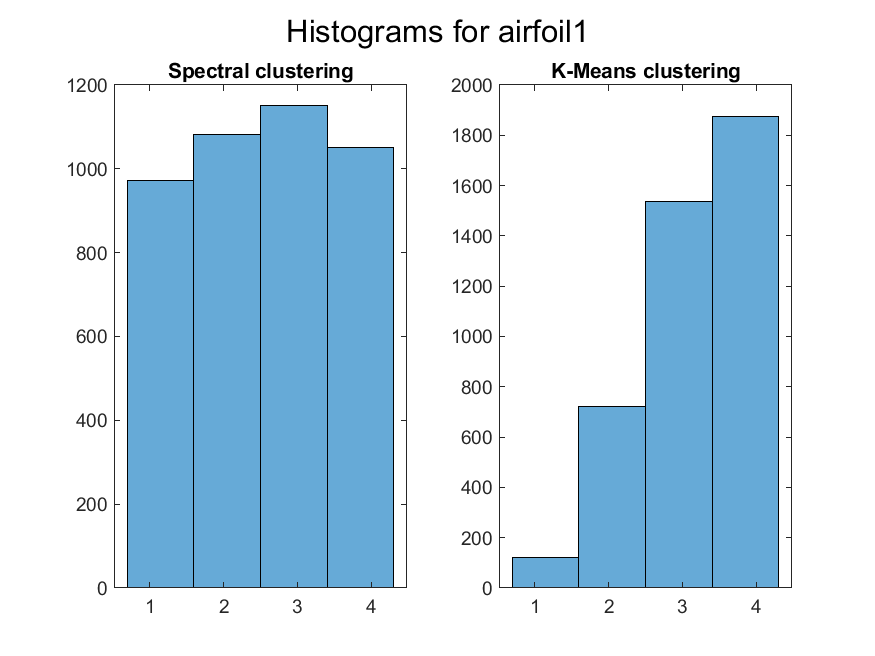
\includegraphics[width=\linewidth]{figures/2.3_airfoil1.png}
        \caption{Airfoil1}
        \label{fig:airfoil1-2.3}
    \end{subfigure}
    \hfill
    \begin{subfigure}{0.45\textwidth}
        \centering
        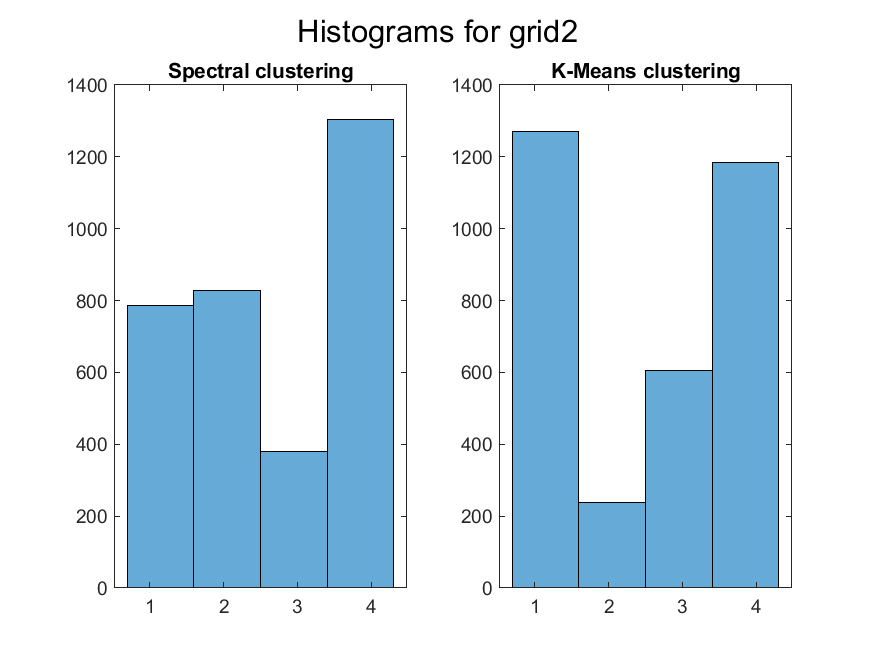
\includegraphics[width=\linewidth]{figures/2.3_grid2.png}
        \caption{Grid2}
        \label{fig:grid2-2.3}
    \end{subfigure}

    \begin{subfigure}{0.45\textwidth}
        \centering
        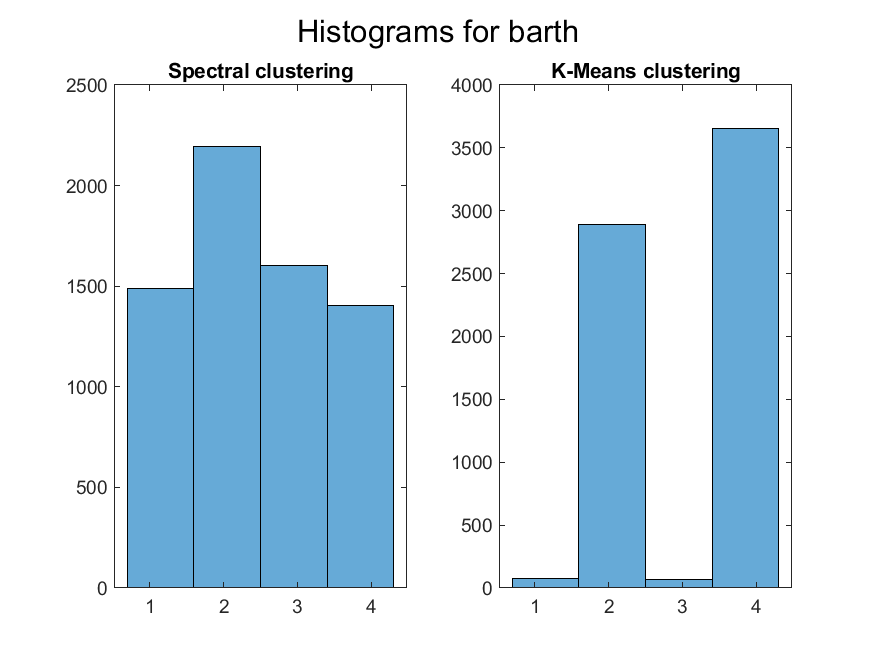
\includegraphics[width=\linewidth]{figures/2.3_barth.png}
        \caption{Barth}
        \label{fig:barth-2.3}
    \end{subfigure}
    \hfill
    \begin{subfigure}{0.45\textwidth}
        \centering
        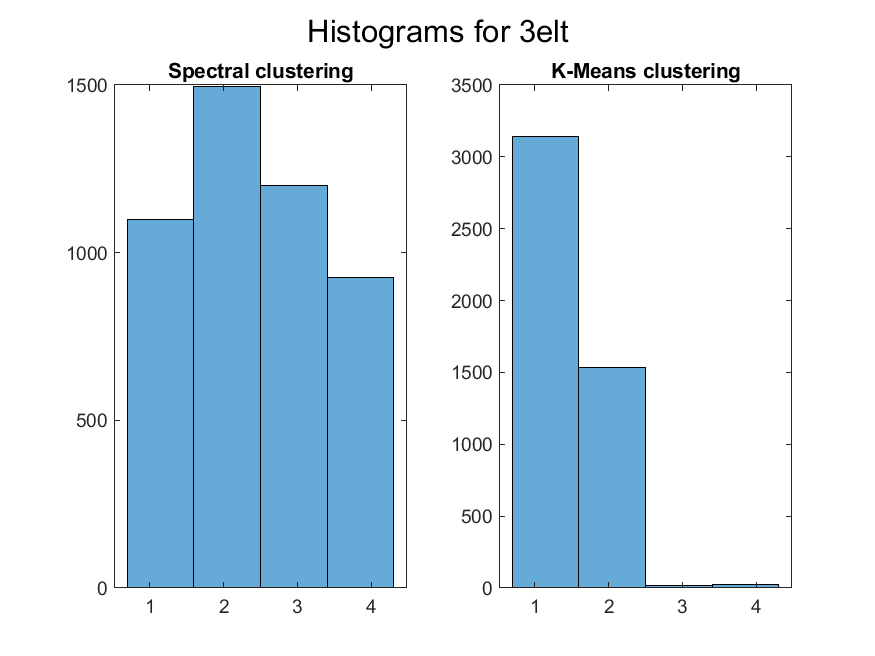
\includegraphics[width=\linewidth]{figures/2.3_3elt.png}
        \caption{3elt}
        \label{fig:3elt-2.3}
    \end{subfigure}
    \caption{Histograms for Different Meshes}
    \label{fig:overall-2.3}
\end{figure}







\end{document}
